\subsection{BenchCouncil AIBench}
{{\footnotesize
\noindent AIBench is a comprehensive benchmark suite that evaluates AI workloads at different levels (micro, component, application) across hardware systems-covering image generation, object detection, translation, recommendation, video prediction, etc.


\begin{description}[labelwidth=4cm, labelsep=1em, leftmargin=4cm, itemsep=0.1em, parsep=0em]
  \item[date:] 2020-01-01
  \item[version:] v1.0
  \item[last\_updated:] 2020-01
  \item[expired:] unknown
  \item[valid:] yes
  \item[valid\_date:] 2020-01-01
  \item[url:] \href{https://www.benchcouncil.org/AIBench/}{https://www.benchcouncil.org/AIBench/}
  \item[doi:] 10.48550/arXiv.1908.08998
  \item[domain:] General
  \item[focus:] End-to-end AI benchmarking across micro, component, and application levels
  \item[keywords:]
    - benchmarking
    - AI systems
    - application-level evaluation
  \item[licensing:] Apache License 2.0
  \item[task\_types:]
    - Training
    - Inference
    - End-to-end AI workloads
  \item[ai\_capability\_measured:]
    - System-level AI workload performance
  \item[metrics:]
    - Throughput
    - Latency
    - Accuracy
  \item[models:]
    - ResNet
    - BERT
    - GANs
    - Recommendation systems
  \item[ml\_motif:]
    - General
  \item[type:] Benchmark
  \item[ml\_task:]
    - NA
  \item[solutions:] Solution details are described in the referenced paper or repository.
  \item[notes:] Covers scenario-distilling, micro, component, and end-to-end benchmarks.

  \item[contact.name:] Wanling Gao (BenchCouncil)
  \item[contact.email:] unknown
  \item[results.links.name:] ChatGPT LLM
  \item[fair.reproducible:] Yes
  \item[fair.benchmark\_ready:] Yes
  \item[id:] benchcouncil\_aibench
  \item[Citations:] \cite{gao2019aibenchindustrystandardinternet}
\end{description}

{\bf Ratings:} ~ \\

\begin{tabular}{p{0.15\textwidth} p{0.07\textwidth} p{0.7\textwidth}}
\hline
Rating & Value & Reason \\
\hline
dataset & 3 & Multiple datasets are mentioned, but not consistently FAIR-documented, versioned, or linked
 \\
documentation & 3 & Paper is comprehensive, but minimal user-facing documentation or structured reproduction guide
 \\
metrics & 4 & Metrics are appropriate, but standardization and reproducibility across tasks vary
 \\
reference\_solution & 3 & Reference models (e.g., ResNet, BERT) described; no turnkey implementation or results repository for all levels
 \\
software & 3 & No containerized or automated implementation provided for full benchmark suite
 \\
specification & 4 & Task coverage is broad and well-scoped, but system constraints and expected outputs are not uniformly defined
 \\
\hline
\end{tabular}

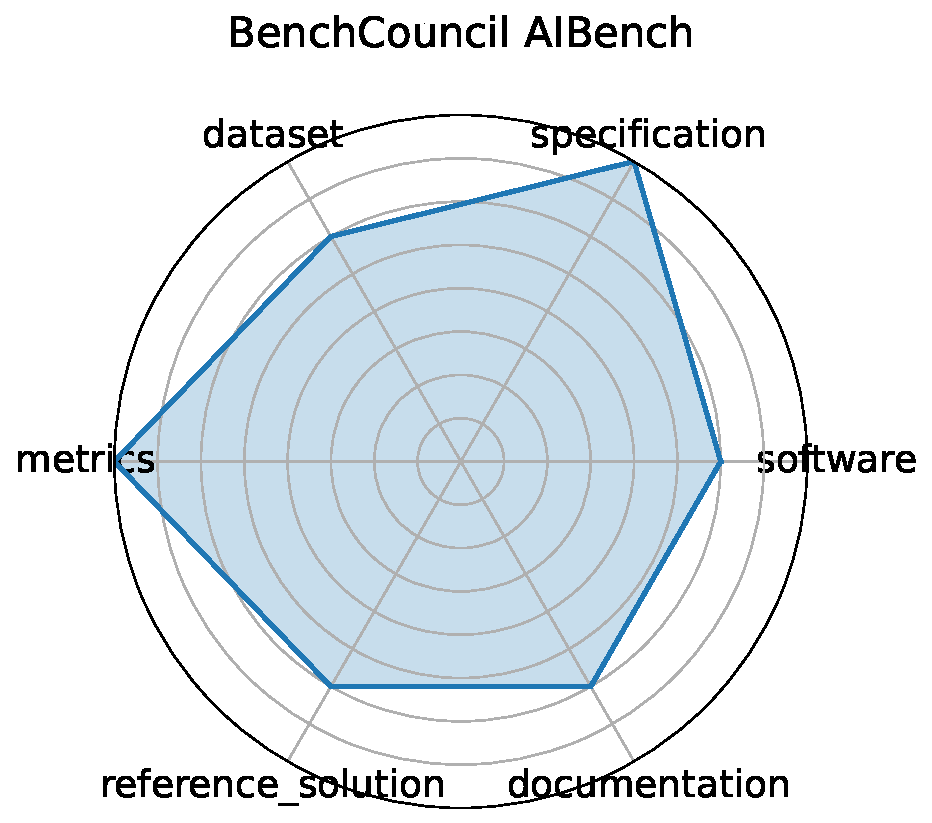
\includegraphics[width=0.2\textwidth]{benchcouncil_aibench_radar.pdf}
}}
\clearpage